\documentclass[11pt]{article}
% Remember to install runcode.sty or copy runcode.sty to the same folder of this file.
\usepackage[run,julia]{runcode}
\usepackage[margin=1in]{geometry}

\begin{document}
\begin{center}\large \bf
  BIST/STAT 4875/5535 - Nonparametric Methods -  Fall 2020 \\
  Homework 1: Solution \\
\end{center}

\begin{enumerate}
\item The result
  \includeOutput{prob1}
  is printed from the following code.
  \showCode{julia}{hw01-1.jl}
  \runJulia{hw01-1.jl}{prob1}
  
\item \runJulia{hw01-2.jl}{prob2}
  The correlation coefficient between $x$ and $y$ is $r=\inlnJulia{```print(corr)```}$, but the scatter plot looks like this:
  \begin{center}
    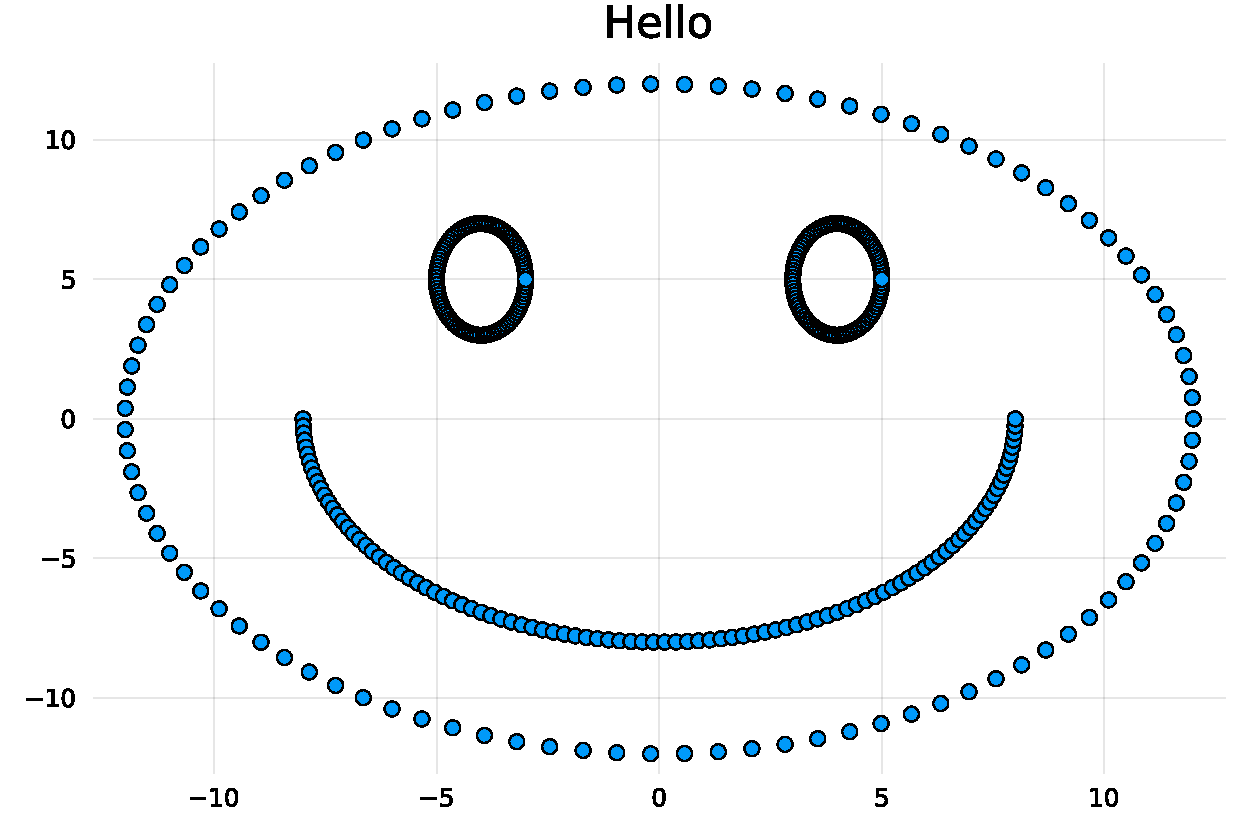
\includegraphics[width=0.5\textwidth]{face.pdf}
  \end{center}
  The computation is performed using the following code
  \showCode{julia}{hw01-2.jl}
\end{enumerate}

\end{document}